\subsection{Observaciones en intervalos, fibras y rectángulos}\label{macro:observaciones}

Tomamos una partición $\mathcal I$ de $[0,1]$ en intervalos de longitud a lo sumo $a_{\rm mac}$, con
extremos
asignados a un solo intervalo. Podemos usar intervalos iguales. Un índice pertenece al intervalo de su
centro físico. Para filas y columnas registramos
\[
 N^R_I=\frac1n\sum_{r_i\in I}X_{R_i},\qquad
 N^C_I=\frac1n\sum_{c_j\in I}X_{C_j},\qquad
 N^{R,*}_I=N^{C,*}_I=x|I|.
\]
En una fila el parámetro de la fibra es $c$. En una columna, diagonal o antidiagonal es $r$. Fijamos
una línea $\lambda$, que llamamos \emph{distinguida}: es la línea cuya fibra se observa. Dado un
intervalo $I$, escribimos $\lambda_I$ para la parte de la fibra física cuyo parámetro pertenece a
$I$, y $dz$ para la medida de ese parámetro. No aparece un factor de
longitud euclídea en las fibras oblicuas, pues hay $n$ índices por unidad de $r$.

\begin{definicion}[Observaciones por fibra]\label{macro:fibras}
Mientras $\lambda$ está disponible, su observación es
\[
 F_{\lambda,I}=\frac1n\sum_{e\in\lambda_I}
                  \prod_{f\ni e,\ f\ne\lambda}X_f .
\]
En cada una de las cuatro familias el objetivo $F^*_{\lambda,I}$ es la integral en $\lambda_I$ de la
densidad de la segunda columna de la tabla. La última columna da la suma de tasas de las tres líneas
que figuran en el producto, antes de dividir por $x$.
\[
\begin{array}{c|c|c}
 \lambda & \text{densidad del objetivo} & H^*_{\lambda}(e)\\ \hline
 R_i & xU_DU_A  & 1+\ell_D^*+\ell_A^*\\
 C_j & xU_DU_A  & 1+\ell_D^*+\ell_A^*\\
 D_d & x^2U_A   & 2+\ell_A^*\\
 A_{a'} & x^2U_D & 2+\ell_D^*
\end{array}
\]
Si la elección del paso ocupa $\lambda$, se conservan los valores de $F_{\lambda,I}$ y
$F^*_{\lambda,I}$ inmediatamente anteriores al paso y se mantienen constantes en adelante. Llamamos
a esto \emph{regla de congelación}. Los balances del Lema~\ref{macro:balances} sólo utilizan líneas
todavía disponibles.
\end{definicion}

Para un rectángulo ordenamos sus posiciones como
$e_1=(i,j)$, $e_2=(i',j)$, $e_3=(i',j')$, $e_4=(i,j')$.
Llamamos ordinaria a la cuádrupla $(i,i',j,j')$ si $i\ne i'$, $j\ne j'$ y las cuatro etiquetas de cada
familia diagonal son distintas entre sí. Las demás cuádruplas son $O(n^3)$. Cada igualdad prohibida es
una ecuación lineal no idéntica en cuatro índices. Fijar tres índices apropiados determina el cuarto,
y sólo hay un número fijo de igualdades. Esta estimación también cubre los bordes del tablero.

\begin{definicion}[Observaciones de rectángulos]\label{macro:rectangulos}
Para $T\subseteq\{1,2,3,4\}$ y una caja $\Theta\in\mathcal I^4$, se siguen la suma y su objetivo
\begin{align*}
 P_{\Theta,T}&=\frac1{n^4}
 \sum_{(i,i',j,j')\in\Theta}^{\rm ord}
 X_{R_i}X_{R_{i'}}X_{C_j}X_{C_{j'}}
 \prod_{m\in T}X_{D(e_m)}X_{A(e_m)},\\
 P^*_{\Theta,T}&=\int_\Theta x^4\prod_{m\in T}U_{D(e_m)}U_{A(e_m)}
                  \,dr\,dr'\,dc\,dc'.
\end{align*}
Las posiciones en la integral se forman con las cuatro coordenadas continuas. El patrón de
$T=\varnothing$ cuenta sólo las dos filas y las dos columnas. Los rectángulos individuales que pierden
una línea dejan de contribuir.
\end{definicion}

Medimos las discrepancias por
\begin{align*}
 \Delta_0&=\sum_{I\in\mathcal I}
   (\bigl|N^R_I-x|I|\bigr|+\bigl|N^C_I-x|I|\bigr|),\\
 \Delta_F&=\max_{\lambda}\sum_{I\in\mathcal I}|F_{\lambda,I}-F^*_{\lambda,I}|,\\
 \Delta_R&=\sum_{\Theta\in\mathcal I^4}\ \sum_{T\subseteq\{1,2,3,4\}}
                      |P_{\Theta,T}-P^*_{\Theta,T}|,\qquad
 \Delta=\Delta_0+\Delta_F+\Delta_R .
\end{align*}
En la primera línea, $x|I|$ es la masa objetivo de cada intervalo. Escribimos $C_{\mathcal I}$ para
constantes
que pueden depender de la partición fija $\mathcal I$ y
\[
 \zeta=\Delta_0+\Delta_F+a_{\rm mac}+C_{\mathcal I}/n .
\]
En las $k$ filas y $k$ columnas disponibles consideramos
\[
 q_{ij}=\frac{Y_{ij}\nu_1(r_i,c_j)}{kU_{D(i,j)}U_{A(i,j)}},\qquad
 V_{ij}=\frac{\nu_1(r_i,c_j)}k .
\]
Los factores $U$ se evalúan en $x$, de modo que $q_{ij}=Y_{ij}W_x(r_i,c_j)/k=Y_{ij}v_x(r_i,c_j)/n$.
La matriz $q$ es el candidato explícito al punto de Bethe: la Proposición~\ref{macro:maximo} prueba
que $p_e/q_e$ está cerca de uno en las casillas disponibles. La matriz $V$ se obtiene de $q$ al
sustituir $Y_{ij}$ por $U_DU_A$, que es su objetivo cuando la fila y la columna están disponibles.

La Figura~\ref{fig:rectangulo} muestra dos posiciones elegidas y el signo que les corresponde.
\begin{figure}[htbp]
\centering
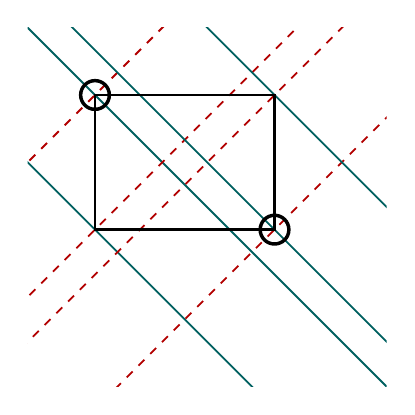
\begin{tikzpicture}[x=.57cm,y=.57cm]
 \bcuadricula{8}
 \begin{scope}
  \clip (0,0) rectangle (8,8);
  \foreach \rr/\cc in {2/2,5/2,5/6,2/6}{
   \draw[teal!75!black,line width=.65pt] ({\cc-.5},{8.5-\rr}) ++(-8,8) -- ++(16,-16);
   \draw[red!70!black,dashed,line width=.65pt] ({\cc-.5},{8.5-\rr}) ++(-8,-8) -- ++(16,16);
  }
 \end{scope}
 \draw[black,line width=1pt] (1.5,6.5) rectangle (5.5,3.5);
 \foreach \rr/\cc in {2/2,5/2,5/6,2/6}{\bmarca{8}{\rr}{\cc}}
 \draw[black,line width=1.25pt] (1.5,6.5) circle[radius=.32];
 \draw[black,line width=1.25pt] (5.5,3.5) circle[radius=.32];
\end{tikzpicture}
\caption{Rectángulo en un tablero vacío de orden ocho. Las filas se numeran desde uno de arriba abajo
y las columnas desde uno de izquierda a derecha. Los vértices en orden son $e_1=(2,2)$, $e_2=(5,2)$,
$e_3=(5,6)$ y $e_4=(2,6)$. Pasan por ellos cuatro diagonales $i-j$ (continuas) y cuatro antidiagonales
$i+j-1$ (discontinuas). Los círculos eligen los vértices opuestos $e_1,e_3$. El término de la
expansión con $T=\{1,3\}$ tiene signo $(-1)^{4-2}=+1$.}\label{fig:rectangulo}
\end{figure}


\begin{lema}[Balances por intervalos y fibras]\label{macro:balances}
Para $k\ge\delta n$, las sumas por filas y por columnas de $V$ difieren de uno en
$O_\delta(\Delta_0+a_{\rm mac}+C_{\mathcal I}/n)$. Las de $q$ difieren de uno y sus masas sobre líneas
diagonales
disponibles difieren de $\ell_f^*$ en
$O_\delta(\Delta_F+a_{\rm mac}+C_{\mathcal I}/n)$, uniformemente en las líneas.
\end{lema}
\begin{proof}
En cada intervalo sustituimos el peso por su valor en un punto de la parte física que se integra. Los
pesos $\nu_1$ y $W_x=\nu_1/(U_DU_A)$ son uniformemente acotados y Lipschitz. El error de la sustitución,
sumado sobre los intervalos de una línea, es $O_\delta(a_{\rm mac})$, pues multiplica la suma de masas
de esa
línea. El error de las masas ponderadas es a lo sumo la norma suprema del peso por la suma de
discrepancias absolutas. La conversión de $1/n$ a $1/k$ aporta $1/x$. Para $V$ el objetivo de una fila
es $x^{-1}\int\nu_1(r,c)x\,dc=1$, y análogamente en las columnas. En una fila disponible, los tres
indicadores del observable de fibra dan $Y_{ij}$ y su masa ponderada objetivo es
\[
 \frac1x\int_0^1 \frac{\nu_1}{U_DU_A}\,xU_DU_A\,dc=1.
\]
La misma cuenta con $dr$ da la suma de una columna. Para la diagonal $d$ el objetivo es
\[
 \frac1x\int_{D_d}\frac{\nu_1}{U_DU_A}\,x^2U_A\,dr
 =\frac{xm_D(d)}{U_D(d)} .
\]
En una antidiagonal se intercambian $D$ y $A$ y resulta $xm_A/U_A$. Las aproximaciones de extremos o
por sumas de Riemann en la partición fija cuestan a lo sumo $C_{\mathcal I}/n$.
\end{proof}
